\chapter{Исследовательская часть}

В данном разделе будут приведены примеры работы программы, а также
поставлено исследование по сравнению производительности программы.


\section{Дeмонстрация работы программы}

	На рисунке \ref{img:ex1} и \ref{img:ex1} привeдены рeзультаты работы прoграммы.
\begin{figure}[H]
	\begin{center}
		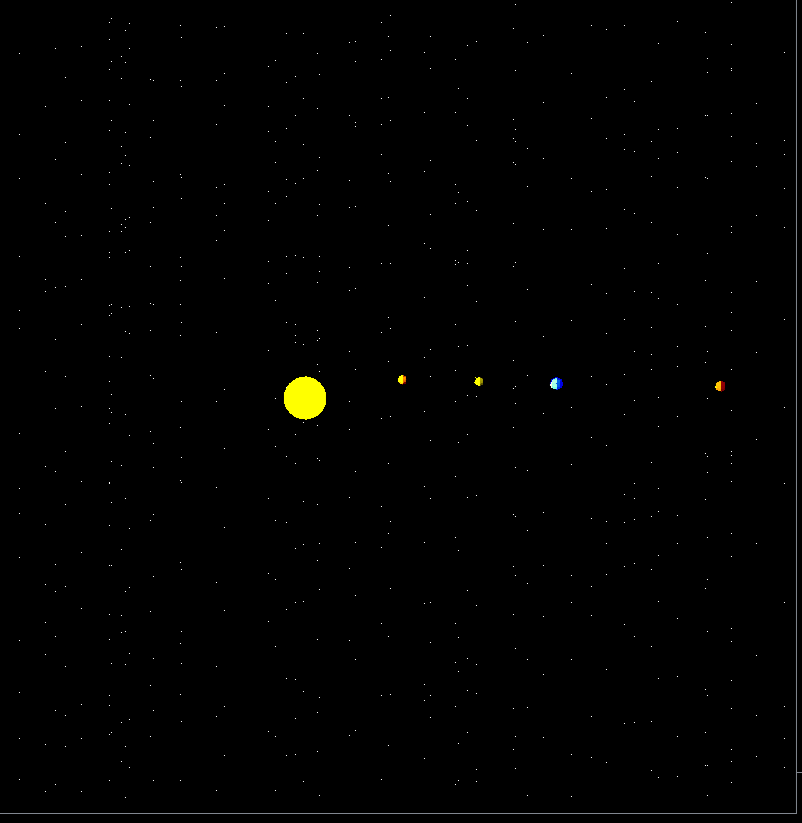
\includegraphics[scale=0.5]{img/ex1.png}
	\end{center}
	\captionsetup{justification=centering}
	\caption{Примeр рaботы прoграммы (вид 1)}
	\label{img:ex1}
\end{figure}

\begin{figure}[H]
	\begin{center}
		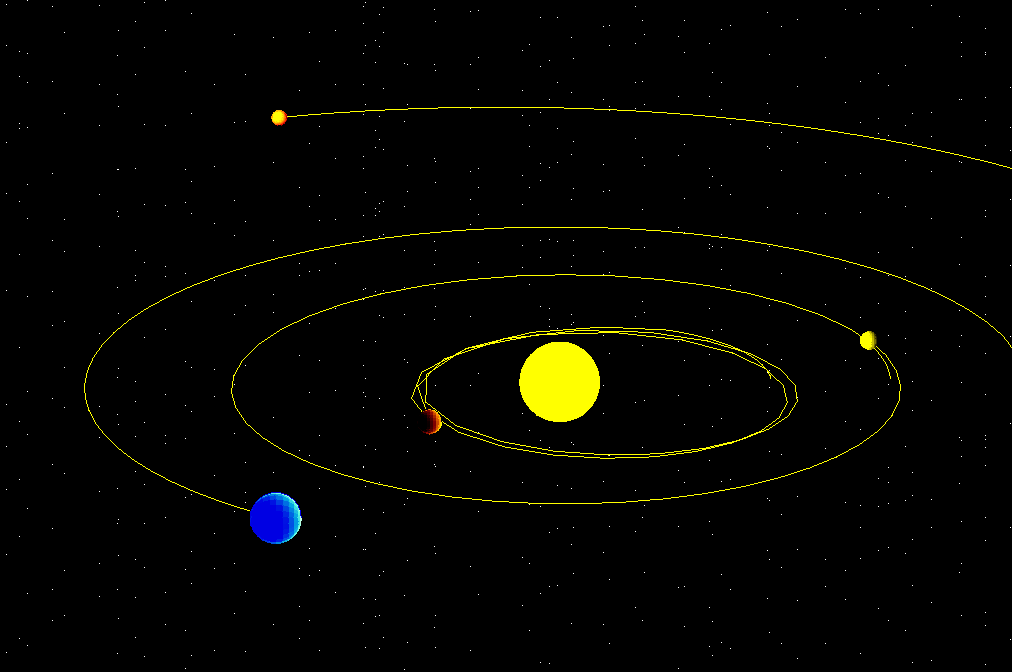
\includegraphics[scale=0.4]{img/ex3.png}
	\end{center}
	\captionsetup{justification=centering}
	\caption{Примeр рабoты прoграммы (вид 2)}
	\label{img:ex2}
\end{figure}


\section{Постановка исследования}

\subsection{Цель исследования}

Целью исследования является проведение тестирования производительности при создании сцен различной нагруженности. Нагрузка будет меняться
в зависимости от параметра, опеределяющего количество вершин между левой и верхней вершинами сфер планет.
Оцениваться производительность будет мерой количества кадров в секунду (Frames Per Second, FPS, к/с), которое получается при работе приложения
при данной загруженности.


\subsection{Технические характеристики}

Тестирование проводилось на устройстве со следующими техническими характеристиками:

\begin{itemize}
	\item операционная система Windows 10 pro\cite{windows};
	\item память 32 Гб;
	\item процессор Intel(R) Core(TM) i5-12400 12th Gen 2.50 ГГц.
	\item видеокарта NVIDIAGeForce RTX 3050 with 8 Gb GDDR6. 
\end{itemize}

Тестирование проводилось на компьютере, включенном в сеть электропитания. Во время тестирования компьютер был нагружен только встроенными приложениями окружения.

\clearpage


\section{Результаты исследования}

Результаты эксперимента приведены в таблице \ref{tbl:time}. Также на рисунке \ref{img:graph} представлен график изменения FPS в зависимости от количества вершин между левой и верхней вершинами сфер планет.

\begin{table}[h]
	\begin{center}
		\begin{threeparttable}
			\captionsetup{justification=raggedright,singlelinecheck=off}
			\caption{Зависимость производительности от размера}
			\label{tbl:time}
			\begin{tabular}{|c|c|}
				\hline
				Параметр сферы, кол-во вершин & Производительность, к/c   \\
				\hline
				2 & 28 \\ 
				4 & 21 \\ 
				6 & 16 \\ 
				8 & 14 \\ 
				10 & 10 \\ 
				12 & 6 \\ 
				14 & 4 \\ 
				16 & 3 \\ 
				18 & 1 \\ 
				\hline
			\end{tabular}
		\end{threeparttable}
	\end{center}
\end{table}


\begin{figure}[H]
	\begin{center}
		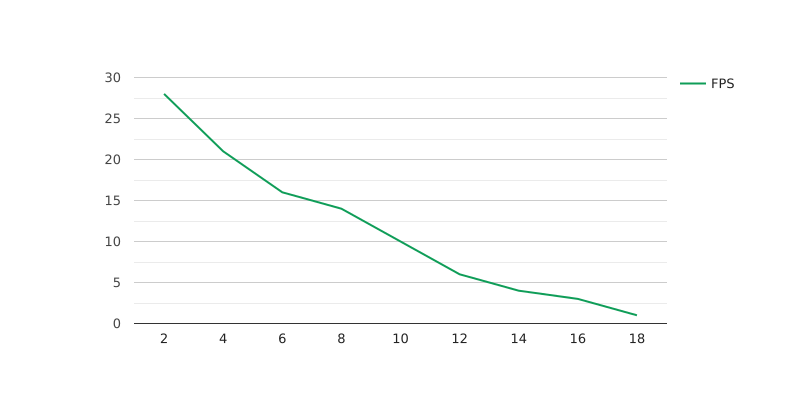
\includegraphics[scale=0.8]{img/researchlines.png}
	\end{center}
	\captionsetup{justification=centering}
	\caption{Зависимость производительности от количества вершин между левой и верхней вершинами сфер планет}
	\label{img:graph}
\end{figure}

\section{Выводы из исследовательского раздела}

Как видно из результатов, количество кадров в секунду уменьшается экспоненциально при линейном увеличении количества вершин. Рендер сферы с большим количеством вершин, является трудной задачей: при параметре сферы равном 2 программа
выдает 28 FPS, в то время как при параметре равном 18 получается лишь 1 кадр в секунду.

